\documentclass[aspectratio=169]{beamer}
\usepackage{spc}
\begin{document}

\begin{frame}
  \title{\darkblue Introduction to Git and GitHub}
  \author{\darkgray\bf Arni Magnusson\\
    \phantom{.}\h{32ex}
\includegraphics[width=1cm]{github_logo}}
  \date{\darkgreen SPC Git/GitHub Workshop\\[0.5ex]
    Noumea, 13 April 2022}
  \titlepage
\end{frame}

% ______________________________________________________________________________

\begin{frame}{Overview}
  \begin{itemize}
    \item[] \hyperlink{examples}{\bf\darkblue Examples}
    \comment{SPC software/analyses/information\\[1ex]
      \h{14ex}fisheries software, open data, personal notes}\\[5ex]
    \item[] \hyperlink{benefits}{\bf\darkblue Benefits}
    \comment{track changes, backups, collaboration, dissemination}\\[5ex]
    \item[] \hyperlink{git}{\bf\darkblue Git concepts}
    \comment{repositories, commits, tags, branches, gitignore}\\[5ex]
    \item[] \hyperlink{github}{\bf\darkblue GitHub features}
    \comment{releases, assets, forks, pull requests, issues,\\[1ex]
      \h{21.4ex}browse, access control, authentication}\\[1ex]
  \end{itemize}
\end{frame}

% ______________________________________________________________________________

\begin{frame}\Large
  \hypertarget{examples}
  \centering\darkgreen\bf
  GitHub Examples
\end{frame}

% ______________________________________________________________________________

\begin{frame}[plain]
  \begin{tikzpicture}[remember picture,overlay]
    \node[at=(current page.center)]
    {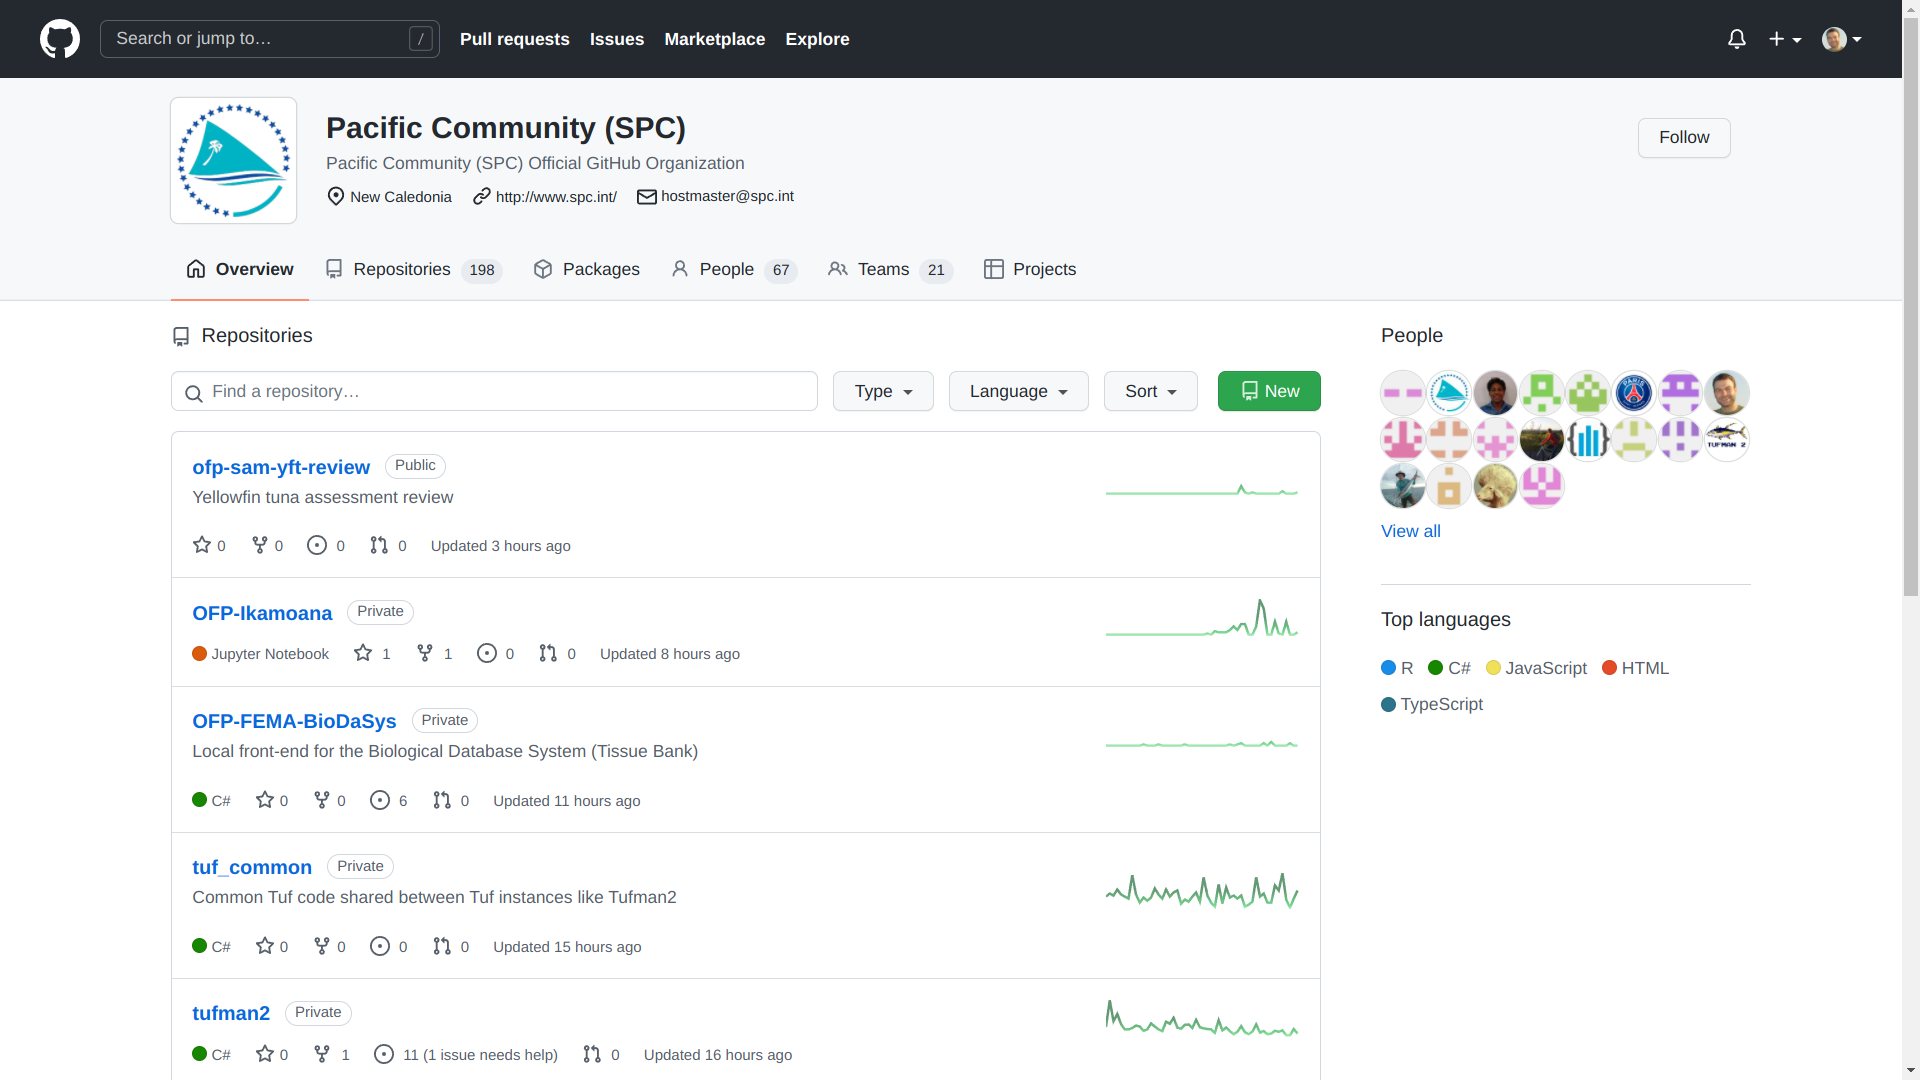
\includegraphics[width=\paperwidth]{github_spc}};
  \end{tikzpicture}
\end{frame}

% ______________________________________________________________________________

\begin{frame}{Repositories}\small\green
  \begin{tabular}{ll}
    \bf\darkblue SPC software
    & \href{https://github.com/PacificCommunity/tufman2}{TUFMAN2},
      \href{https://github.com/PacificCommunity/ofp-md2}{MD2},
      \href{https://github.com/PacificCommunity/ofp-sam-mfcl}{MFCL},
      \href{https://github.com/PacificCommunity/ofp-sam-mfcl-viewer}
      {MFCL viewer},
      \href{https://github.com/PacificCommunity/ofp-sam-flr4mfcl}{FLR4MFCL},
      \href{https://github.com/PacificCommunity/ofp-sam-latex-utils}
      {LaTeX utilities}\\[4ex]
    \bf\darkblue SPC analyses
    & \href{https://github.com/PacificCommunity/ofp-sam-cpue2021}
      {CPUE analysis},
      \href{https://github.com/PacificCommunity/ofp-sam-yft-2020-runs}
      {Yellowfin 2020 assessment},
      \href{https://github.com/PacificCommunity/ofp-sam-skj22}
      {Skipjack 2022 assessment}\\[4ex]
    \bf\darkblue SPC information
    & \href{https://github.com/PacificCommunity/ofp-sam-yft-review}
      {Yellowfin review},
      \href{https://github.com/PacificCommunity/ofp-sam-htcondor}
      {Condor tutorial},
      \href{https://github.com/PacificCommunity/ofp-sam-institutional-memory}
      {Condor notes},
      \href{https://github.com/PacificCommunity/ofp-sam-taf-demo}
      {TAF demo}\\[4ex]
    \bf\darkblue Fisheries software
    & \href{https://github.com/admb-project/admb}{ADMB},
      \href{https://github.com/kaskr/adcomp}{TMB},
      \href{https://github.com/James-Thorson-NOAA/VAST}{VAST},
      \href{https://github.com/fishfollower/SAM}{SAM},
      \href{https://github.com/gadget-framework/gadget2}{Gadget},
      \href{https://github.com/NIWAFisheriesModelling/CASAL2}{CASAL},
      \href{https://github.com/nmfs-stock-synthesis/stock-synthesis}
      {Stock Synthesis},
      \href{https://github.com/ices-tools-prod/TAF}{TAF}\\[4ex]
    \bf\darkblue Open data
    & \href{https://github.com/cfree14/wcfish}{US West Coast fisheries},
      \href{https://github.com/CSSEGISandData/COVID-19}{Covid data}\\[4ex]
    \bf\darkblue Personal notes
    & \href{https://github.com/arni-magnusson/corona}{Covid analysis},
      \href{https://github.com/arni-magnusson/dot}{Computer settings}
  \end{tabular}
\end{frame}

% ______________________________________________________________________________

\begin{frame}\Large
  \hypertarget{benefits}
  \centering\darkgreen\bf
  Benefits of Using Git and GitHub
\end{frame}

% ______________________________________________________________________________

\begin{frame}{Benefits}\small
  \begin{description}
    \item[\bf Track changes] Who changed what, when, and why\\[5ex]
    \item[\bf Backups] Online\\[1ex]
    Restore previous state\\[5ex]
    \item[\bf Collaboration] Local, regional, international\\[1ex]
    \h{1ex}Software development, analyses, other projects\\[5ex]
    \item[\bf Dissemination] Software\\[1ex]
    \h{1.5ex}Open science, data hub\\[1ex]
    \h{1.5ex}Products\\[1ex]
  \end{description}
\end{frame}

% ______________________________________________________________________________

\begin{frame}\Large
  \hypertarget{git}
  \centering\darkgreen\bf
  Git Concepts
\end{frame}

% ______________________________________________________________________________

\begin{frame}{Git and GitHub}\small
  {\bf\darkblue Git}\\[-1ex]
  \begin{itemize}
    \item[] A program \comment{that you can install}\\[0.8ex]
    \item[] Version control software \comment{tracking changes}\\[0.8ex]
    \item[] Load and save project snapshots \comment{clone, commit}\\[0.8ex]
    \item[] Free software \comment{created by Linus Torvalds in 2005}\\[4ex]
  \end{itemize}
  {\bf\darkblue GitHub}\\[-1ex]
  \begin{itemize}
    \item[] A website \comment{open `\href{https://github.com}{github.com}' in a
      browser}\\[0.8ex]
    \item[] Service for Git projects \comment{pull requests, issues}\\[0.8ex]
    \item[] Browse online \comment{view changes, download}\\[0.8ex]
    \item[] Basic functionality is free \comment{created 2008, owned by
      Microsoft since 2018}\\[4ex]
  \end{itemize}
  \darkgray\it\fns Popular in fisheries science since around 2015
\end{frame}

% ______________________________________________________________________________

\begin{frame}{Git Concepts}\small
  \begin{description}
    \item[\bf\darkblue Repository] Project folder with tracked changes
    \comment{a sequence of commits}\\[5ex]
    \item[\bf\darkblue Commit] Saved snapshot \comment{example: bc4b374}\\[5ex]
    \item[\bf\darkblue Tag] Nickname for a significant commit \comment{example:
      2.0.0}\\[5ex]
    \item[\bf\darkblue Branch] Parallel sequence of commits \comment{can be
      merged later with the main branch}\\[5ex]
    \item[\bf\darkblue Gitignore] List of local files that should be ignored
    \comment{not uploaded to repository}
  \end{description}
\end{frame}

% ______________________________________________________________________________

\begin{frame}\Large
  \hypertarget{github}
  \centering\darkgreen\bf
  GitHub Features
\end{frame}

% ______________________________________________________________________________

\begin{frame}{GitHub Features}
  Release
  Assets
  Forks
  Pull request
  Issue
\end{frame}

% ______________________________________________________________________________

\begin{frame}{GitHub Features (cont)}
  Browse
  Access control
  Authentication
\end{frame}

\end{document}
